
\subsection{Analyse Telekom}
Auf allen Seiten ist die Navigation konstant gehalten. In der Navigation ist ein fehlender alternativer Text beim Logo (Abbildung 4.22) und damit ist dieser Fehler auch auf jeder Seite. 

\begin{figure}[H]
    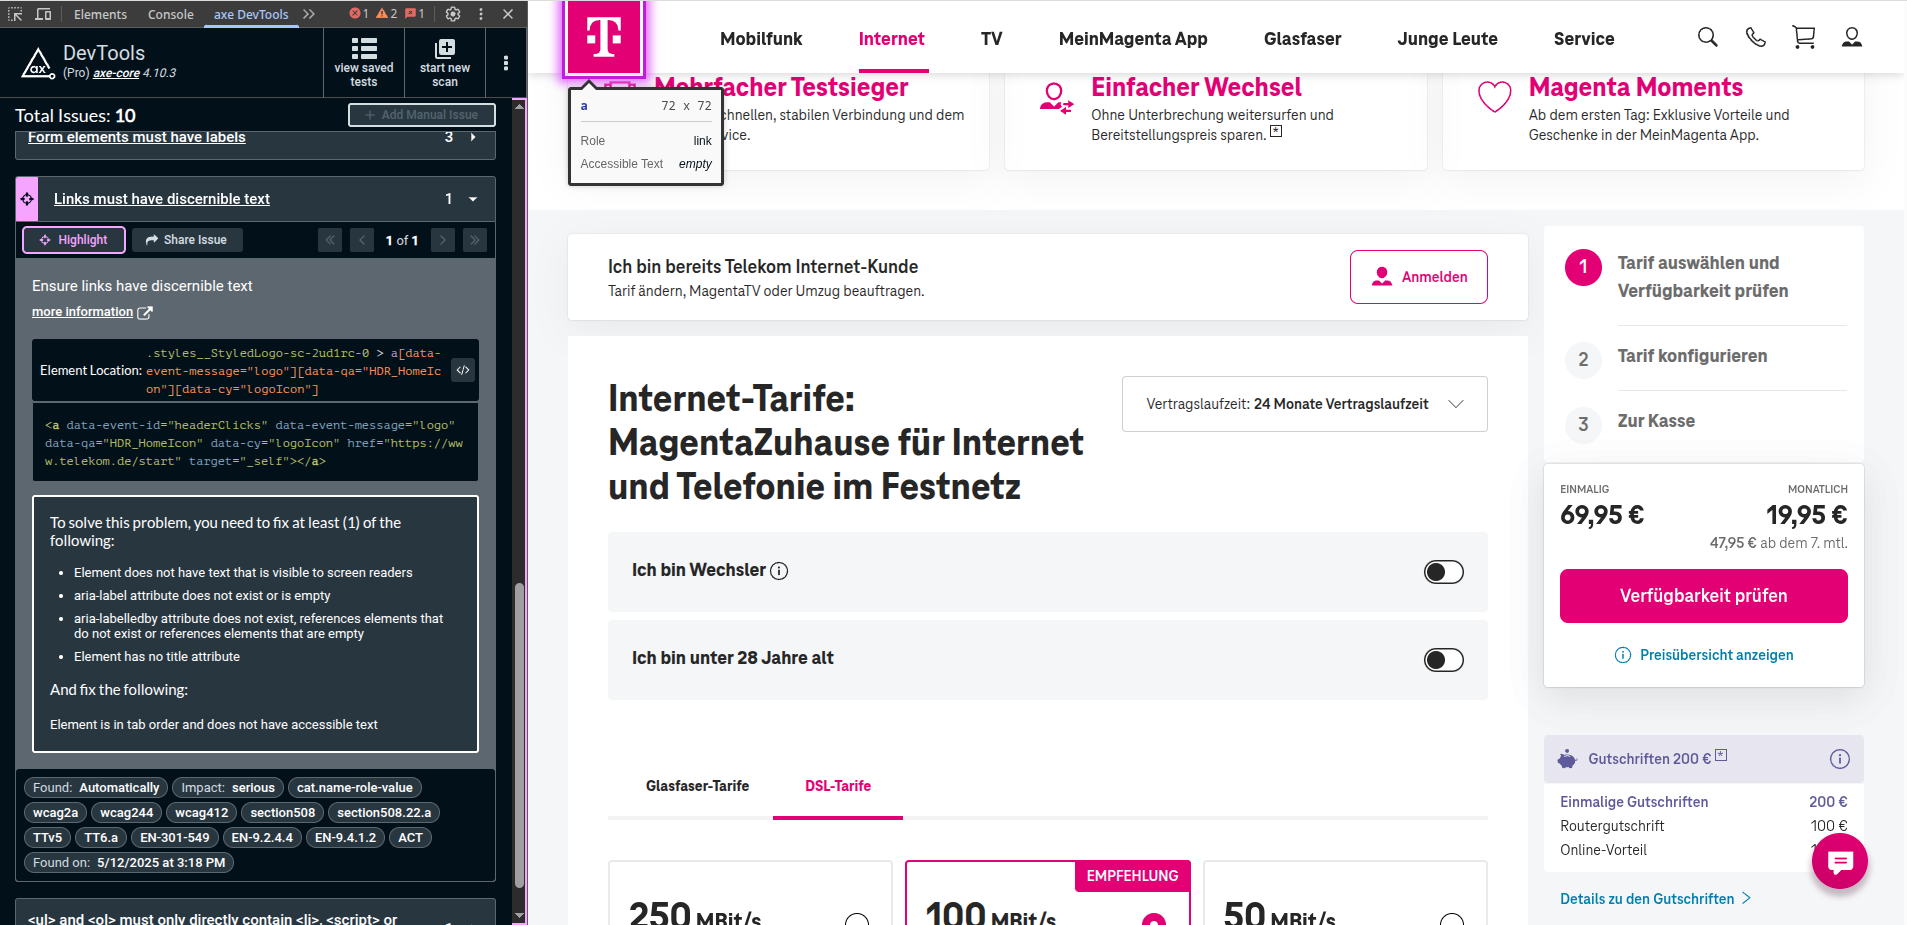
\includegraphics[width=\textwidth]{img/telekom_no-alt-text_logo.png}
    \caption{Fehlender alternativer Text}
\end{figure}

Sonst findet man auf der Startseite keine Fehler, bis auf einem fehlendem sichtbaren Fokus von zwei Checkboxen. 

\begin{figure}[H]
    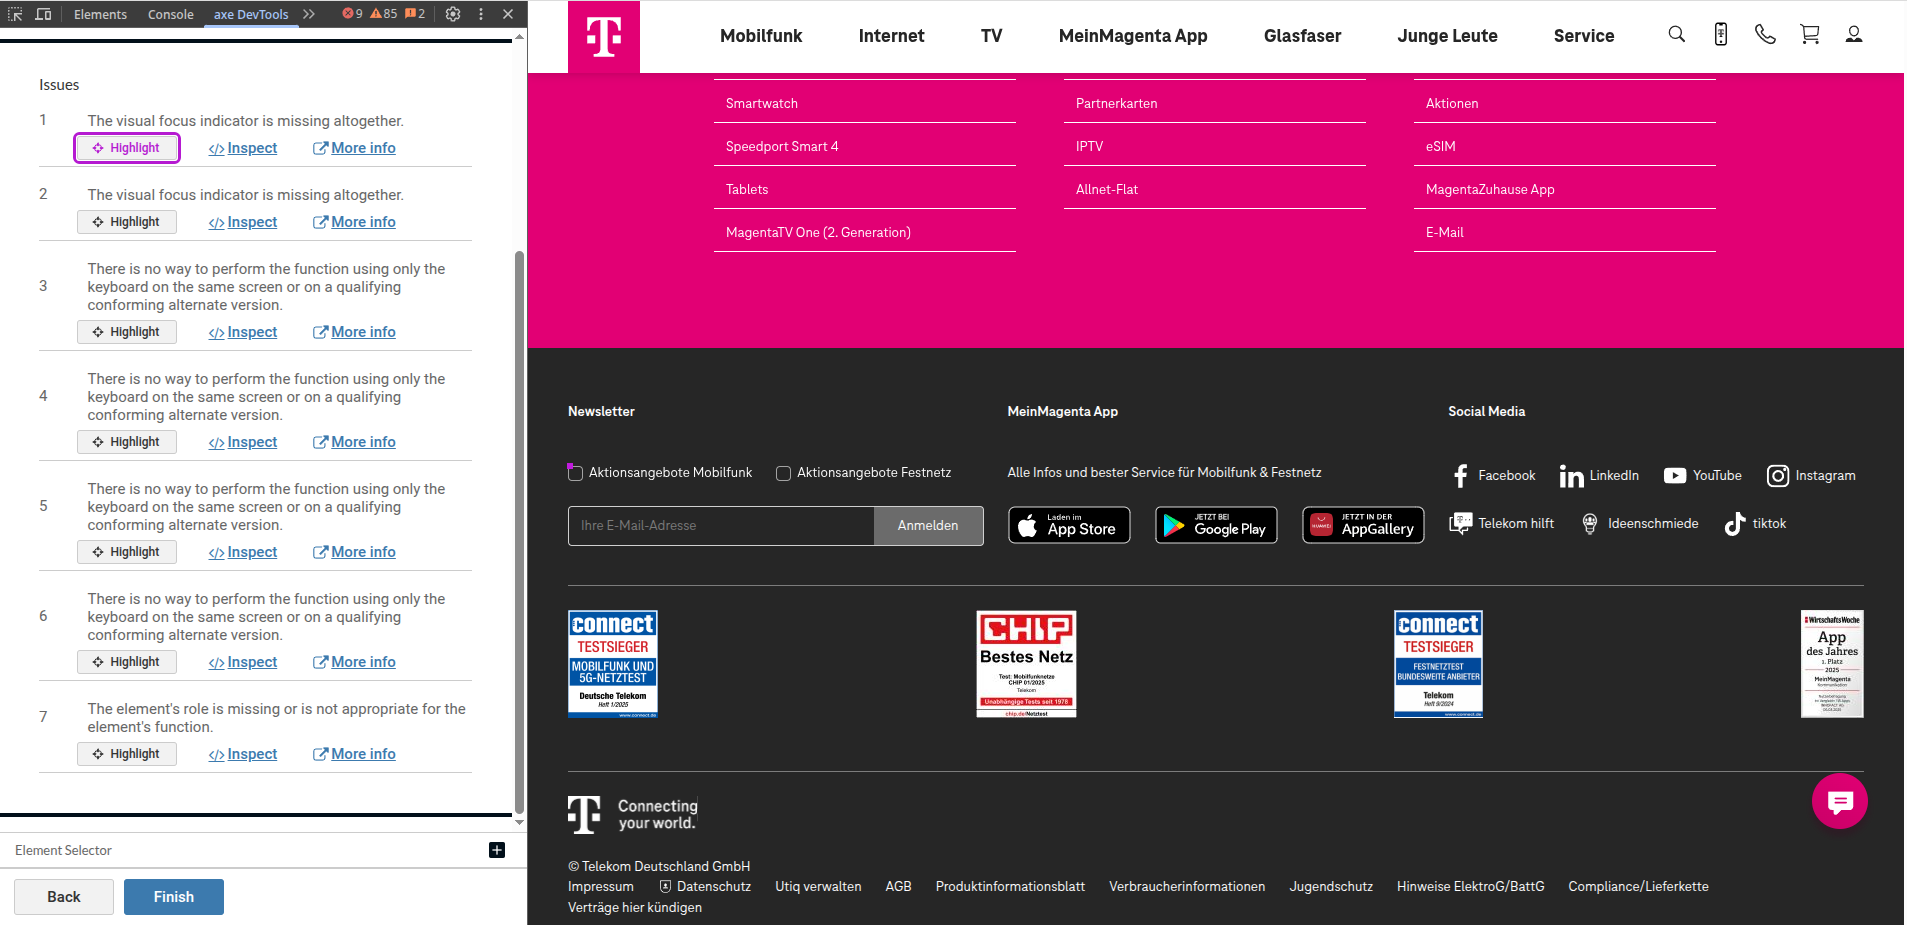
\includegraphics[width=\textwidth]{img/telekom_checkbox-no-focus.png}
    \caption{Fehlende Fokussierung bei Checkboxen}
\end{figure}

Außerdem wurde die Verfügbarkeit-Seite untersucht, um zu sehen, ob man sich auch ohne Barriere Informationen einholen kann. Dabei wurde festgestellt, dass die Seite nicht vollständig barrierefrei ist. 

Die Verfügbarkeit lässt sich über ein PopUp-Fenster abfragen. Dabei hat der Schließen-Button kein Aria-Label und ist damit nicht korrekt benannt.

\begin{figure}[H]
    
\includegraphics[width=\textwidth]{img/telekom_no-aria-label_close-button.png}
    \caption{Fehlendes Aria-Label bei einem Schließen-Button}
\end{figure}

Dazu haben die Input-Felder, in denen ich die Adresse eingeben kann, kein Label. Dies ist ein Verstoß gegen Kriterium 4.1.2 \enquote{Name, Rolle, Wert}.
\begin{figure}[H]
    
\includegraphics[width=\textwidth]{img/telekom_no-label.png}
    \caption{Fehlendes Label bei einem Eingabefeld}
\end{figure}

Die Breadcrumb-Navigation, die helfen soll, sich auf der Seite zurecht zu finden, ist nicht korrekt umgesetzt. Es ist als Liste angelegt, aber die einzelnen Listenelemente sind keine semantisch richtigen Kind-Elemente. Anstelle eines <li> wurde ein <span> verwendet. Dies ist ein Verstoß gegen Kriterium 1.3.1 \enquote{Info und Beziehungen}.

\begin{figure}[H]
    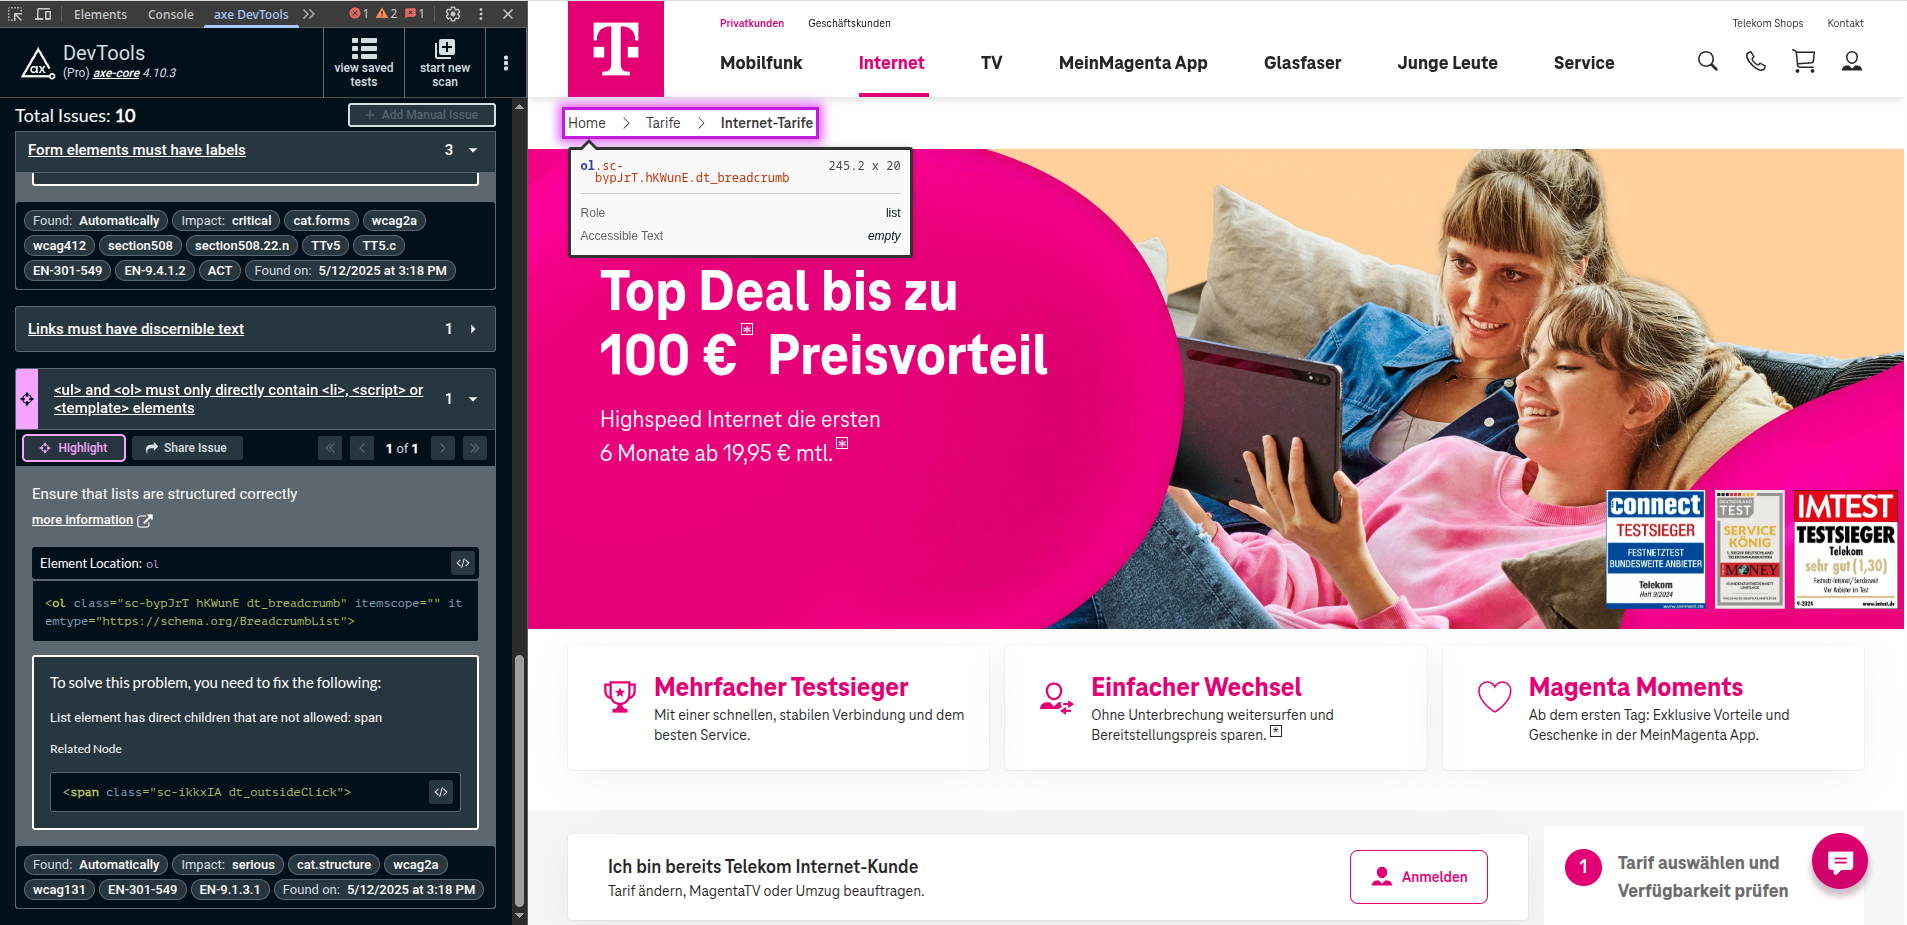
\includegraphics[width=\textwidth]{img/telekom_ol-no-li.png}
    \caption{Breadcrumb-Navigation}
\end{figure}

Die Varianz an unterschiedlichen Fehlern ist bei der Telekom wieder geringer. Allerdings sind die Fehler, die auftreten, auch auf anderen Seiten zu finden. So ist der Fehler mit dem fehlenden alternativen Text bei dem Logo auch auf der Startseite und auf der Verfügbarkeit-Seite zu finden. Auch die Breadcrumb-Navigation ist auf mehreren Seiten zu finden.

\begin{figure}[H]
\begin{tikzpicture}
\begin{axis}[
    width=\textwidth,
    height=10cm,
    ybar,
    bar width=12pt,
    xlabel={WCAG-Kriterium},
    ylabel={Fehleranzahl},
    symbolic x coords={ 9.1.1.1, 9.1.3.1, 9.1.4.3, 9.2.4.1, 9.2.4.4, 9.2.4.7, 9.4.1.2 },
    xtick=data,
    x tick label style={rotate=45, anchor=east},
    ymin=0,
    ymax=350,
    enlarge x limits=0.1,
    legend style={cells={anchor=west}, legend pos=north east},
    nodes near coords,
    nodes near coords style={font=\scriptsize},
]
\addplot table[x=WCAG-Kriterium,y=Fehleranzahl_axe,col sep=tab]{csv/output/wcag_analyse_Telekom_xxxx.csv};
\addplot table[x=WCAG-Kriterium,y=Fehleranzahl_WAVE,col sep=tab]{csv/output/wcag_analyse_Telekom_xxxx.csv};
\legend{axe,WAVE}
\end{axis}
\end{tikzpicture}
\caption{Auswertung Analyse Telekom}
\end{figure}
